
\chapter{Introduction}
\label{ch:introduction}

The objective of the Semantic Web vision is to enable data from heterogeneous datasources to be interconnected in order to establish a Global Information Source. 
The Resource Description Framework (RDF) is a common modeling language used for developing ontolgies to conceptualize and represent information about existing resources in the Semantic Web.
In addition, a number of software applications from diverse fields, such as Big Data, Machine Learning, and Data Science, are generating data from their legacy systems in the RDF language. 
On the other hand, new applications are developed relying their data management mechanisms completely on RDF.
To facilitate the exchanging of data between software applications, several serializations formats, such as RDF{/}XML, Turtle, N-Triples, and JSON-LD \footnote{\url{https://www.w3.org/TR/rdf-syntax-grammar/}, \url{https://www.w3.org/TR/turtle/}, \url{https://www.w3.org/TR/n-triples/}, and \url{https://www.w3.org/2018/jsonld-cg-reports/json-ld/}}, have been proposed over the years.
These formats address different requirements, such that: 1) RDF{/}XML is tailored for parsing with existing XML tools and libraries; 2) Turtle, for being more human-readable; 3) N-Triples aims at simplifying parsing procedures; and 4) JSON-LD, to allow encoding of the RDF data in the JSON format.
A fundamental pre-condition to consume the RDF data encoded in so-called RDF documents, is that they are syntactically correct.
Several approaches are presented to deal with the syntax validation of the RDF documents.
However, most available approaches which check for syntactic errors in RDF fail to detect more than one error at the same time, in particular when data are serialized in Turtle or N-Triples format, respectively. 
Therefore, we observe a need for an approach able to identify all syntactic errors simultaneously which allow producing of qualitative RDF documents from the syntactic perspective.

In this thesis, we present RDF-Doctor, a comprehensive approach for error detection and correction of RDF documents.
The motivation of this study was mainly encouraged by the  tremendous RDF data representation and usage in both Turtle and N-Triples serialization formats.
RDF-Doctor is capable of detecting an exhaustive number of syntactic errors, particularly, in Turtle or N-Triple format, respectively. 
In addition, our approach is able to automatically correct a subset of already found errors.
Additionally, RDF-Doctor offers user-friendly messages to facilitate manual correction for common and frequently encountered errors, such as missing a colon or a dot, or a non-defined prefix.  

%The following text in this chapter are divided in a couple of sections to express our motivation of the study, present the problem statement, presents the challenges, list our research contributions, and finally outline how this thesis is structured.  

\section{Motivation}

%This study was motivated by real world application where exists demand for dealing wit, have as a requirement for their operating, syntax checking of RDF data when it comes as an input. 
Let us suppose a group of users, Bob, Hani, and Sarah, are working together in developing an ontology for representing the knowledge about a particular domain as illustrated in Figure~\ref{Fig:Motivation}.
The ontology will be used in a data processing system to support classification and analysis of data generated from heterogeneous sources. 
Since all involved users are experienced ontology engineers, they prefer to realize the ontology development using plain text editors.
To exchange and distribute their changes, they use a version control system, such as Git \footnote{\url{https://git-scm.com/}}.
Any change made to ontology is initially verified against syntax errors. Where in the case of found errors, the system will stop processing the input data and return a report of errors to the user. 
Existing tools used for syntax checking, assert that the input is syntax-error-free. 
If the ontology has more than one error, these tools naturally stop parsing and report only the first error to the user with other information about the error, such as an error message, row and column number, and where the error occurred.

Probably, an ontology after each change may have more than one syntactic error.
The procedure of correcting them is as follows: When the first error is encountered, the system reports the error.
Thereafter the user reads the error message and locates the error within the ontology file. 
Next, the user corrects the error and resubmits its version with recent modifications.
The system checks for syntax and again detects another error, causing to the user to repeat the same procedure of error correction.
This will continue until the ontology file is free of errors.
However, it might happen that during the correction phase users can introduce new errors.
Therefore, this procedure is time consuming, error-prone, and tedious to all involved users in the ontology development process.
%Subsequently, the reported error is commonly corrected by the user to be sent again for re-checking of the syntax. To make it more complex, suppose the user has 10 syntax errors in his RDF input, then, the previous process steps of an input checking, an pause of parsing, an error notifying, and an error correction by the user has to be repeated for 10 times.  Furthermore, when the number of syntax errors increases, the number of error processing and correction processes increases by the same value. Also, imagine what is the consumed time and the work overload to process an input RDF data contains hundreds or thousands of errors.  

	\begin{figure}[ht]
			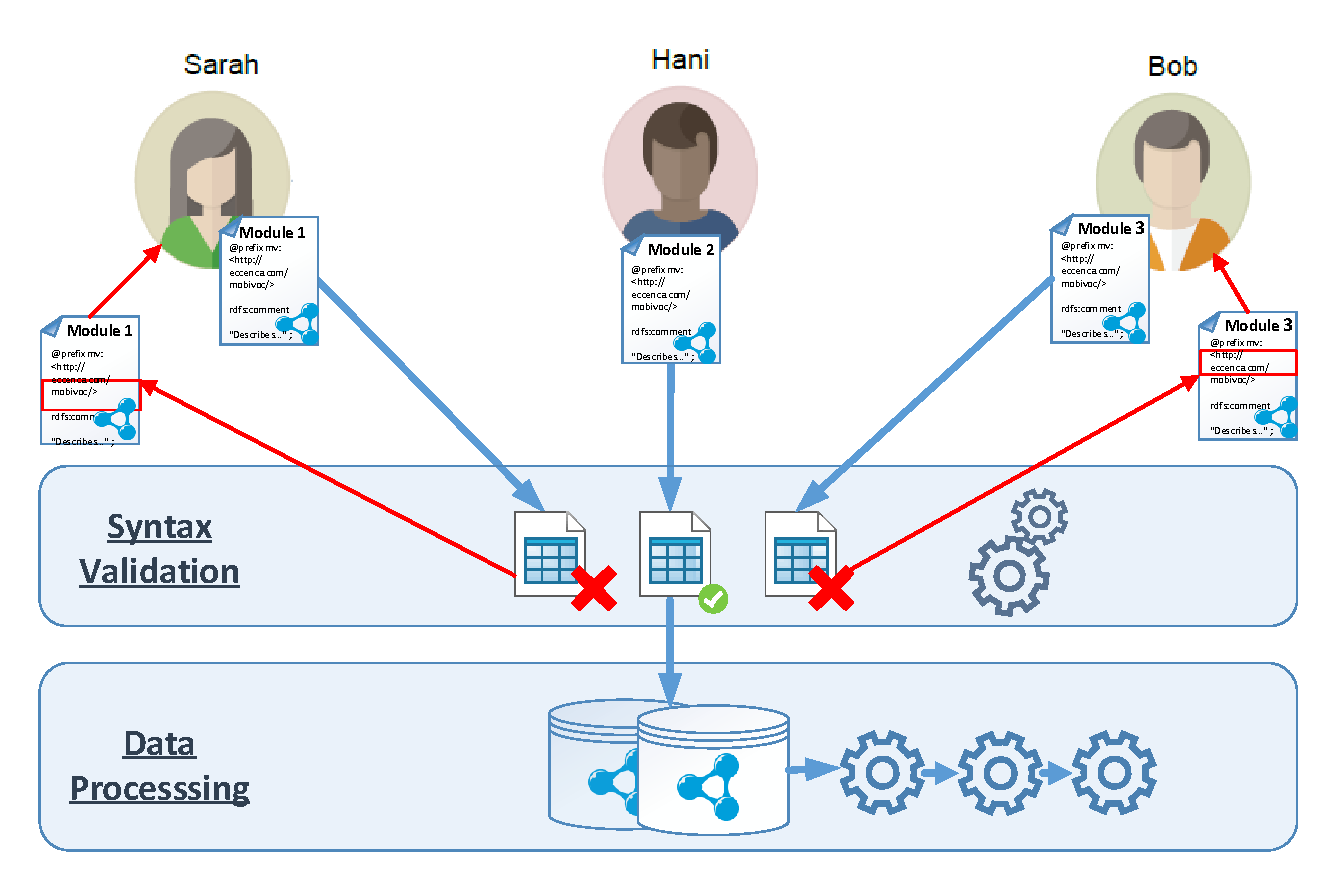
\includegraphics[width=0.9\textwidth]{images/motivation.pdf}
			\caption{\textbf{Motivation example.} A typical scenario where different ontology engineers send their ontology versions to the system for syntax validation before further data processing.
			Both Sarah and Bob have one or more syntax errors, but they receive one error at time and they have to manually resolve it.
			On the other hand,  Hani's version passed with no syntax errors and went to the next phase for further processing.}
			\label{Fig:Motivation}
	\end{figure}

%let's dig deep in demonstrating what is there in  {Figure \ref{Fig:Motivation}}, It is showing a flow of data from clients or users seeking further data processing. 3 persons are shown in this Figure, their names are Bob, Hani, and Sarah. All of them start with the first phase by sending their data to be syntactically checked. The parser starts checking if there are syntax errors of the input data, if such data passed with no syntax errors, it can be forwarded for further phases, i.e. for data processing, otherwise, the input data will send back to the user to correct the errors. {Figure \ref{Fig:Motivation}} clearly shows that Sarah and Bob have syntax errors in their input data,then, they got an error report, including details about the first detected error. In the meanwhile, Hani has received his data processed without getting such a report, since his input data has no syntax errors. 

%This study has been fostered by the former illustrated example to find a suitable solution to allow the parser to continue the whole input of RDF data checking against syntax error and to list them in an error report if any was found. Therefore, the proposed solution focuses on producing a software tool that can detect all syntax errors that can be detected in the input RDF data. 

%\section{Objectives}
\section{Problem Description and Challenges} 	
Ideally, ontology engineers should be able to retrieve and easily correct any existing error in their ontology version.
At the conceptual level, this thesis addresses the problem of comprehensive and simultaneous error detection and resolving for RDF documents.
Therefore, the approach should assist ontology engineers on identifying syntactic issues and automatically fix them.
In addition, for any error that is not possible to automatically correct, a user-friendly and understandable message should be provided.

%Before reaching the proposed solution, different methods have been tired to reach the objective. 
Over the year several approaches have been presented for parsing RDF documents and finding syntactic errors.
%The main purpose was the continuation of parsing till the end of the file without stopping on the first syntax error detection  and storing details of the detected errors into a data structure, such as lists. 
Well-known tools, such as: Jena API \cite{McBride:2002:JSW:613357.613755}; RDF4J API \cite{RDF4J:Online}; and N3 Parser \cite{N3Parser:Online}, implemented as Java-based toolkits or as a Javascript-based parser, respectively, are used to process the N-Triple and Turtle serialization formats. 
Commonly, these tools utilize an exception handling mechanism to catch any potential syntax error and are able to recognize only one error at particular time.

We identified several challenges that should be tackled in order to achieve a comprehensive error coverage for RDF documents.
These challenges include: 1) finding the exact position in a given RDF document, where there error is occurring; 2) enabling the continuation of the parsing procedure after encountering of each error; 3) identifying multiple errors in the same line or subsequent statements; 4) automatic correction of a subset of errors; and 5) improving conflict resolution via user-friendly messages.
%Our task was to remove the text that contains the first detected syntax error from an input text (since those tools fail when the first syntax error is found), then, to supply the remaining text for further parsing. 
%Two methods were used: 1) cutting only the triple or the statement that contains the syntax error, 2) removing text before the found syntax error, including the statement of the error. 
%Both those methods were failed to offer a suitable solution for continuation of parsing after an error discovery, for the following reasons: 1) the difficulty of handling nearby syntax errors, such as errors in the same line or in subsequent statements follow each others, 2) the inexpressive and incomprehensible of error messages, especially, in the second tool, which complicates understanding the actual syntax error for further handling.    


%TODO need references.


\section {Contributions}
%In this study, the research work set out to syntactically check RDF data. 
The main contributions of the proposed approach are listed in the following:
\begin{enumerate}
	\item  {\bf Identifying existing syntax errors in RDF Documents:} This is a major goal and contribution with the intention to investigate RDF Documents and search for potential syntax errors. 
	The proposed approach is powered by ANTLR framework \cite{ANTLR:Website:Online}, a powerful parser generator, with the objective of establishing an RDF parser that enables simultaneous listing of all discovered syntax errors. 
	The fundamental aspect of the approach is the injection of the grammar identification rules inside the parser. 
	Once, the parser detects a presence of so-called tokens in an RDF input matching one of the given grammar rules that represent a syntax error, it sends an error notification to the error listener component, where error lists are stored.
	\item {\bf Reporting syntax errors with user-friendly and expressive messages:} Either normal users or ontology engineers are assisted with meaningful error messages. 
	Following the principle from the ancient Greek philosopher, Socrates: “Understanding a question is half an answer”\cite{Socrates:quote:Online}, similarly, an understandable error message helps to recover from an error. 
	Our approach is based on both the regular expression and grammar rules, where each rule represents either a sequence of correct syntax tokens or a sequence of incorrect ones. 
	In the case of the latter, we encoded  predefined information about each error, hence, a customized error message can be formulated in a meaningful and convenient way and delivered on-the-fly to the error listener.  
	\item {\bf Automatic error recovery of a subset of syntax errors:} This includes syntax errors similar to those in well-know programming languages, such as missing a dot, adding more than one dots, or missing a semicolon. 
	A particular rule is designed to limit repeatable conflict notifications while correcting errors and to control the eligibility of an error to be corrected. 
	The rule is to check for the presence of a specific error in a predefined error correction list.
	It includes fundamentally common errors with information about the necessary actions for recovery procedure. 
	For instance, missing a dot or a semicolon are common mistakes during editing of RDF Documents, and these errors can automatically corrected by our approach.
	However, there exists several errors such as missing of a prefix declaration, that cannot be corrected since the details of that missing prefix are obscure and unknown.     
\end{enumerate}

\section {Thesis Structure}
The thesis is structured into seven chapters. 
%Until this spot, \textbf{Chapter \ref{ch:introduction}} was presented, titled with "Introduction". 
It starts with the \emph{Introduction}, where a general overview of the study, the motivation, the problem description and the challenges, as well as contributions are presented. 
The remainder of the thesis is organized as follows:
\begin{itemize}
	\item { \textbf{Chapter \ref{ch:preliminaries}:} Describes the background knowledge which comprises relevant concepts and terminology required to understand the work that has been conducted in this thesis.}
	
	\item {\textbf{Chapter \ref{ch:related}:}} Discusses the existing approaches from the state of the art related parsing of the RDF documents. 
		
	\item {\textbf{Chapter \ref{ch:approach}:}} Presents the proposed approach along with its distinctive characteristics and important features. 
	
	\item {\textbf{Chapter \ref{ch:implementation}:}} Demonstrates the actual implementation of our approach, including the architecture and its modules.
	
	\item {\textbf{Chapter \ref{ch:evaluation}:}} Shows the evaluation part where the approach is tested in three different scenarios and the obtained results are discussed.

	\item {\textbf{Chapter \ref{ch:conclusions}:}} 
	Presents the conclusion of our work realized in this thesis and provides a number of potential future directions.
\end{itemize}







